\chapter{Architecture}\label{arch}
This chapter proposes an architecture for the Trusted Execution Module. The
design is driven by the goal of making it possible to manufacture the TEM at very low
cost, which is required if the TEM is to become a commodity. The text in this
chapter makes heavy use of the concepts presented in chapter \ref{concepts}. My
design was probably biased by the prototype implementation on the JavaCard
platform, so it is likely that some of the details will change if the TEM is
implemented directly on a hardware chip.

The main components of the TEM are the execution engine, the cryptographic
engine, and the persistent store. Figure \ref{fig:tem_overview} contains the
(obligatory) block diagram for the platform. The grayed out components are
not mandatory, but their presence can optimize various aspects of the TEM's
functionality.

\begin{figure}[hbtp]
	\center{
		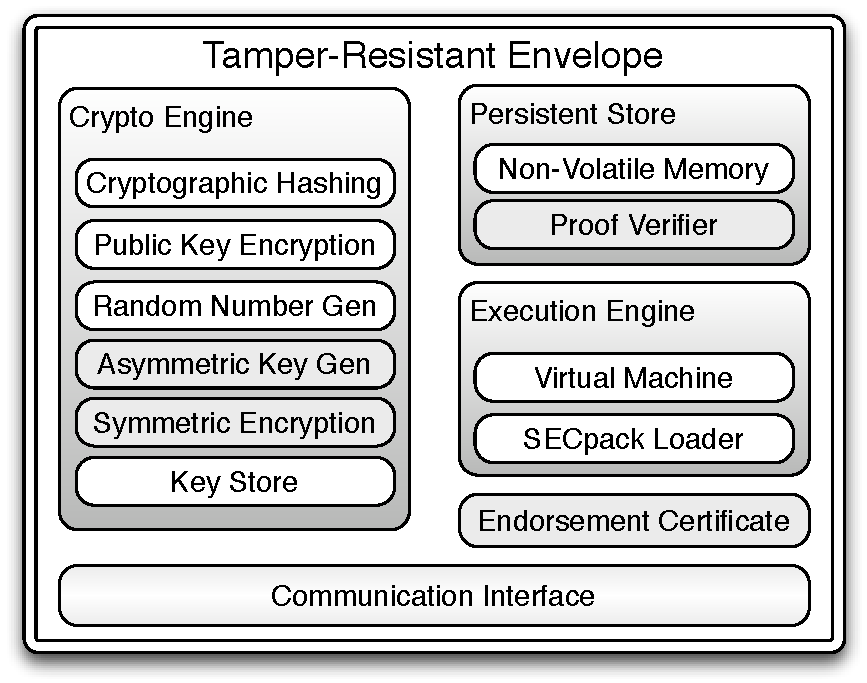
\includegraphics{omnifigs/tem_overview}
	}
	\caption{High-Level TEM Block Diagram}
	\label{fig:tem_overview}
\end{figure}

The TEM's cryptographic engine, covered in section \ref{arch:crypto}, is the
foundation of the TEM's security. The engine must provide random number
generation, cryptographic hashing\footnote{Cryptographic hashes are best
known in the context of digital signatures, where they are sometimes called
message digests.}, and asymmetric key encryption.

Section \ref{arch:execution} describes the TEM's execution engine, which
consists of a SECpack loader, and a stack-based virtual machine. The SEClosure code, local variables, and constant non-local variables are stored in the same flat addressing space. Encryption keys are stored by the cryptographic engine, and they are accessible via special-purpose instructions.

Mutable non-local variables are stored in the (intuitively named) persistent
store, whose design is covered in section \ref{arch:pstore}.

Aside from the main components described above, the TEM also contains a
communication interface, which is described in section \ref{arch:interface}.
The interface serves as an intermediary between the TEM's engines and the
outside world. The interface plays a distinct part when the communication
between the TEM and its owner occurs via untrusted channels, and needs to be secured.

The TEM must be accompanied by driver software which runs on the host computer.
For the sake of completeness, section \ref{arch:driver} summarizes the main
issues in the design of the driver software.
